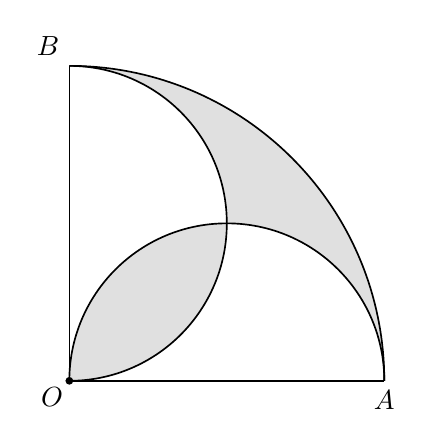
\begin{tikzpicture}[x=1cm,y=1cm,line width=.6pt,font=\normalsize]
\coordinate (O) at (0,0);
\coordinate (A) at (4,0);
\coordinate (B) at (0,4);
\coordinate (Q) at (2,2);
\fill[black!12] (O)--(A) arc[start angle=0,end angle=90,radius=4cm]--cycle;
\fill[white] (O) arc[start angle=180,end angle=0,radius=2cm]--cycle;
\fill[white] (O) arc[start angle=270,end angle=450,radius=2cm]--cycle;
\begin{scope}
\clip (O) arc[start angle=180,end angle=0,radius=2cm]--cycle;
\fill[black!12] (O) arc[start angle=270,end angle=450,radius=2cm]--cycle;
\end{scope}
\draw (O)--(A);
\draw (O)--(B);
\draw (A) arc[start angle=0,end angle=90,radius=4cm];
\draw (O) arc[start angle=180,end angle=0,radius=2cm];
\draw (O) arc[start angle=270,end angle=450,radius=2cm];
\node[below left=2pt,inner sep=0pt] at (O) {$O$};
\node[below] at (A) {$A$};
\node[above left] at (B) {$B$};
\fill (O) circle[radius=1.4pt];
\end{tikzpicture}
